         \chapter{Longitudinal waves}
    \setcounter{figure}{1}
    \setcounter{subfigure}{1}
    \label{e91550bed2a1600e0ddb2572d580bf8e}
         \section{ Introduction and key concepts}
    \nopagebreak
            \label{m38782} $ \hspace{-5pt}\begin{array}{cccccccccccc}   
\includegraphics[width=0.75cm]{col11305.imgs/summary_fullmarks.png} &   \end{array} $ \hspace{2 pt}\raisebox{-5 pt}{} {(section shortcode: P10046 )} \par 
    \label{m38782*cid2}
            \subsection{ Introduction}
            \nopagebreak
      \label{m38782*id291765}We have already studied transverse pulses and waves. In this chapter we look at another type of wave called \textsl{longitudinal} waves. In transverse waves, the motion of the particles in the medium were perpendicular to the direction of the wave. In longitudinal waves, the particles in the medium move \textsl{parallel} (in the \textsl{same} direction as) to the motion of the wave. Examples of transverse waves are water waves or light waves. An example of a longitudinal wave is a sound wave.\par 
    \label{m38782*cid3}
            \subsection{ What is a \textsl{longitudinal wave}?}
            \nopagebreak
\par
            \label{m38782*fhsst!!!underscore!!!id64}\begin{definition}
	  \begin{tabular*}{15 cm}{m{15 mm}m{}}
	\hspace*{-50pt}  
\includegraphics[width=0.5in]{col11305.imgs/psflag2.png}   & \Definition{   \label{id2444157}\textbf{ Longitudinal waves }} { \label{m38782*meaningfhsst!!!underscore!!!id64}
      A longitudinal wave is a wave where the particles in the medium move parallel to the direction of propagation of the wave. 
       } 
      \end{tabular*}
      \end{definition}
      \label{m38782*id292159}When we studied transverse waves we looked at two different motions: the motion of the particles of the medium and the motion of the wave itself. We will do the same for longitudinal waves.\par 
      \label{m38782*id292164}The question is how do we construct such a wave?\par 
      \label{m38782*id292167}To create a transverse wave, we flick the end of for example a rope up and down. The particles move up and down and return to their equilibrium position. The wave moves from left to right and will be displaced.\par 
      \label{m38782*id292172}
    \setcounter{subfigure}{0}
	\begin{figure}[H] % horizontal\label{m38782*id292175}
    \begin{center}
    \label{m38782*id292175!!!underscore!!!media}\label{m38782*id292175!!!underscore!!!printimage}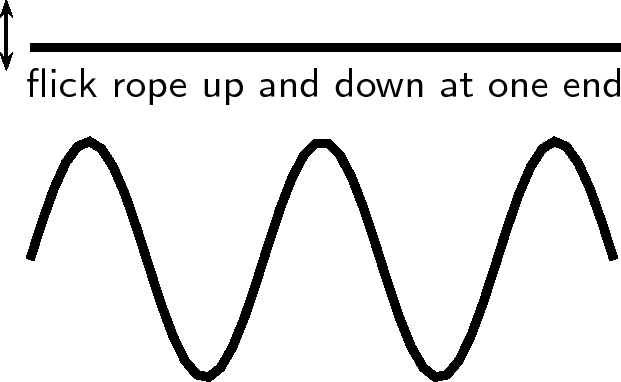
\includegraphics[width=0.4\columnwidth]{col11305.imgs/m38782_PG11C4_001.png} % m38782;PG11C4\_001.png;;;6.0;8.5;
      \vspace{2pt}
    \vspace{.1in}
    \end{center}
 \end{figure}       
      \par 
      \label{m38782*id292181}A longitudinal wave is seen best in a spring that is hung from a ceiling. Do the following investigation to find out more about longitudinal waves.\par 
\label{m38782*secfhsst!!!underscore!!!id79}
            \subsubsection{  Investigation : Investigating longitudinal waves }
            \nopagebreak
      \label{m38782*id292193}\begin{enumerate}[noitemsep, label=\textbf{\arabic*}. ] 
            \label{m38782*uid1}\item Take a spring and hang it from the ceiling. Pull the free end of the spring and release it. Observe what happens.
    \setcounter{subfigure}{0}
	\begin{figure}[H] % horizontal\label{m38782*id292211}
    \begin{center}
    \label{m38782*id292211!!!underscore!!!media}\label{m38782*id292211!!!underscore!!!printimage}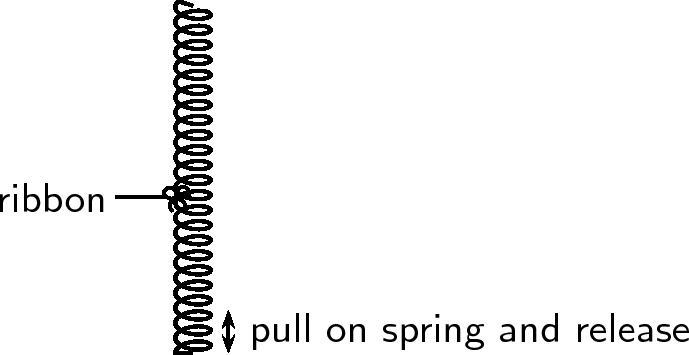
\includegraphics[width=0.55\columnwidth]{col11305.imgs/m38782_PG11C4_002.png} % m38782;PG11C4\_002.png;;;6.0;8.5;
      \vspace{2pt}
    \vspace{.1in}
    \end{center}
 \end{figure}       \label{m38782*uid2}\item In which direction does the disturbance move?
\label{m38782*uid3}\item What happens when the disturbance reaches the ceiling?
\label{m38782*uid4}\item Tie a ribbon to the middle of the spring. Watch carefully what happens to the ribbon when the free end of the spring is pulled and released. Describe the motion of the ribbon.
\end{enumerate}
      \label{m38782*id292264}From the investigation you will have noticed that the disturbance moves parallel to the direction in which the spring was pulled. The spring was pulled down and the wave moved up and down. The ribbon in the investigation represents one particle in the medium. The particles in the medium move in the same direction as the wave. The ribbon moves from rest upwards, then back to its original position, then down and then back to its original position.\par 
    \setcounter{subfigure}{0}
	\begin{figure}[H] % horizontal\label{m38782*uid5}
    \begin{center}
    \rule[.1in]{\figurerulewidth}{.005in} \\
        \label{m38782*uid5!!!underscore!!!media}\label{m38782*uid5!!!underscore!!!printimage}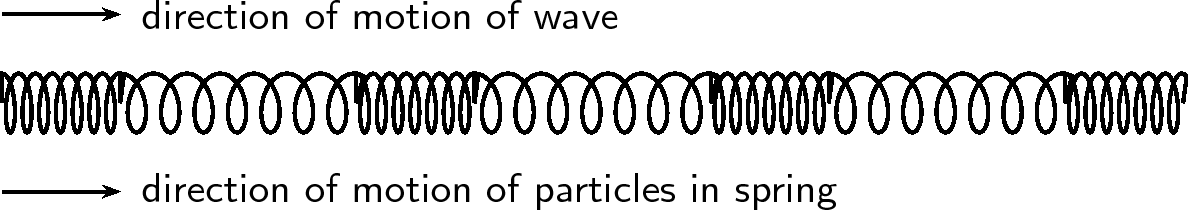
\includegraphics[width=0.8\columnwidth]{col11305.imgs/m38782_PG11C4_003.png} % m38782;PG11C4\_003.png;;;6.0;8.5;
      \vspace{2pt}
    \vspace{\rubberspace}\par \begin{cnxcaption}
	  \small \textbf{Figure 8.3: }Longitudinal wave through a spring
	\end{cnxcaption}
    \vspace{.1in}
    \rule[.1in]{\figurerulewidth}{.005in} \\
    \end{center}
 \end{figure}       
    \label{m38782*cid4}
            \subsection{ Characteristics of Longitudinal Waves}
            \nopagebreak
      \label{m38782*id292291}As in the case of transverse waves the following properties can be defined for longitudinal waves:
wavelength, amplitude, period, frequency and wave speed. However instead of peaks and troughs, longitudinal waves have \textsl{compressions} and \textsl{rarefactions}.\par 
\label{m38782*fhsst!!!underscore!!!id105}\begin{definition}
	  \begin{tabular*}{15 cm}{m{15 mm}m{}}
	\hspace*{-50pt}  
\includegraphics[width=0.5in]{col11305.imgs/psflag2.png}   & \Definition{   \label{id2399629}\textbf{ Compression }} { \label{m38782*meaningfhsst!!!underscore!!!id105}
      A \textbf{compression} is a region in a longitudinal wave where the particles are closest together. 
       } 
      \end{tabular*}
      \end{definition}
\par
            \label{m38782*fhsst!!!underscore!!!id108}\begin{definition}
	  \begin{tabular*}{15 cm}{m{15 mm}m{}}
	\hspace*{-50pt}  
\includegraphics[width=0.5in]{col11305.imgs/psflag2.png}   & \Definition{   \label{id2399653}\textbf{ Rarefaction }} { \label{m38782*meaningfhsst!!!underscore!!!id108}
      A \textbf{rarefaction} is a region in a longitudinal wave where the particles are furthest apart. 
       } 
      \end{tabular*}
      \end{definition}
      \label{m38782*uid6}
            \subsubsection{ Compression and Rarefaction}
            \nopagebreak
        \label{m38782*id292360}As seen in Figure~8.4, there are regions where the medium is compressed and other regions where the medium is spread out in a longitudinal wave.\par 
        \label{m38782*id292369}The region where the medium is compressed is known as a \textbf{compression} and the region where the medium is spread out is known as a \textbf{rarefaction}.\par 
    \setcounter{subfigure}{0}
	\begin{figure}[H] % horizontal\label{m38782*uid7}
    \begin{center}
    \rule[.1in]{\figurerulewidth}{.005in} \\
        \label{m38782*uid7!!!underscore!!!media}\label{m38782*uid7!!!underscore!!!printimage}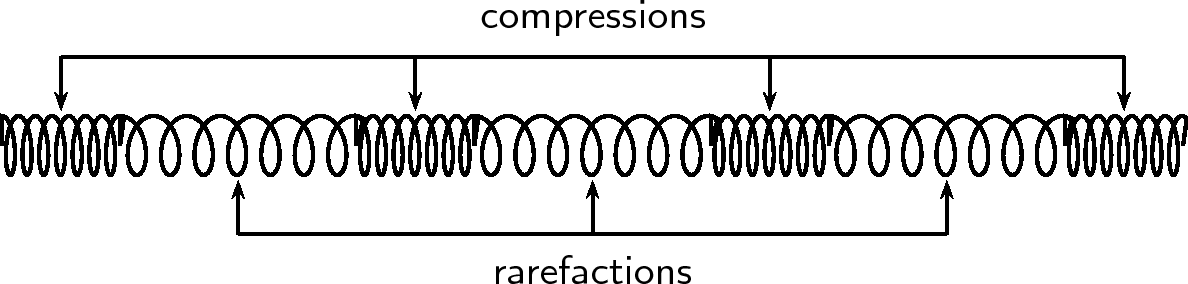
\includegraphics[width=0.8\columnwidth]{col11305.imgs/m38782_PG11C4_004.png} % m38782;PG11C4\_004.png;;;6.0;8.5;
      \vspace{2pt}
    \vspace{\rubberspace}\par \begin{cnxcaption}
	  \small \textbf{Figure 8.4: }Compressions and rarefactions on a longitudinal wave
	\end{cnxcaption}
    \vspace{.1in}
    \rule[.1in]{\figurerulewidth}{.005in} \\
    \end{center}
 \end{figure}       
      \label{m38782*uid8}
            \subsubsection{ Wavelength and Amplitude}
            \nopagebreak
\par
            \label{m38782*fhsst!!!underscore!!!id125}\begin{definition}
	  \begin{tabular*}{15 cm}{m{15 mm}m{}}
	\hspace*{-50pt}  
\includegraphics[width=0.5in]{col11305.imgs/psflag2.png}   & \Definition{   \label{id2445839}\textbf{ Wavelength }} { \label{m38782*meaningfhsst!!!underscore!!!id125}
        The \textbf{wavelength} in a longitudinal wave is the distance between two consecutive points that are in phase. 
         } 
      \end{tabular*}
      \end{definition}
        \label{m38782*id292427}The wavelength in a longitudinal wave refers to the distance between two consecutive compressions or between two consecutive rarefactions.\par 
\label{m38782*fhsst!!!underscore!!!id129}\begin{definition}
	  \begin{tabular*}{15 cm}{m{15 mm}m{}}
	\hspace*{-50pt}  
\includegraphics[width=0.5in]{col11305.imgs/psflag2.png}   & \Definition{   \label{id2445871}\textbf{ Amplitude }} { \label{m38782*meaningfhsst!!!underscore!!!id129}
        The \textbf{amplitude} is the maximum displacement from equilibrium. For a longitudinal wave which is a pressure wave this would be the maximum increase (or decrease) in pressure from the equilibrium pressure that is cause when a peak (or trough) passes a point.
         } 
      \end{tabular*}
      \end{definition}
    \setcounter{subfigure}{0}
	\begin{figure}[H] % horizontal\label{m38782*uid9}
    \begin{center}
    \rule[.1in]{\figurerulewidth}{.005in} \\
        \label{m38782*uid9!!!underscore!!!media}\label{m38782*uid9!!!underscore!!!printimage}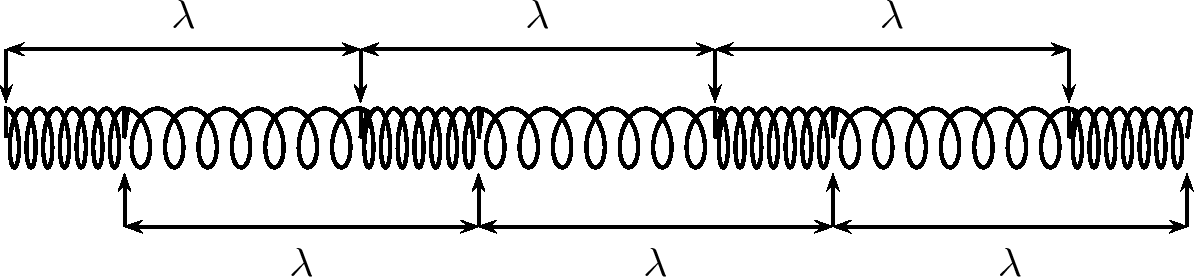
\includegraphics[width=0.8\columnwidth]{col11305.imgs/m38782_PG11C4_005.png} % m38782;PG11C4\_005.png;;;6.0;8.5;
      \vspace{2pt}
    \vspace{\rubberspace}\par \begin{cnxcaption}
	  \small \textbf{Figure 8.5: }Wavelength on a longitudinal wave
	\end{cnxcaption}
    \vspace{.1in}
    \rule[.1in]{\figurerulewidth}{.005in} \\
    \end{center}
 \end{figure}       
        \label{m38782*id292465}The amplitude is the distance from the equilibrium position of the medium to a compression or a rarefaction.\par 
      \label{m38782*uid10}
            \subsubsection{ Period and Frequency}
            \nopagebreak
            \par
            \label{m38782*fhsst!!!underscore!!!id143}\begin{definition}
	  \begin{tabular*}{15 cm}{m{15 mm}m{}}
	\hspace*{-50pt}  
\includegraphics[width=0.5in]{col11305.imgs/psflag2.png}   & \Definition{   \label{id2445953}\textbf{ Period }} { \label{m38782*meaningfhsst!!!underscore!!!id143}
       The \textbf{period} of a wave is the time taken by the wave to move one wavelength.
         } 
      \end{tabular*}
      \end{definition}
\par
            \label{m38782*fhsst!!!underscore!!!id146}\begin{definition}
	  \begin{tabular*}{15 cm}{m{15 mm}m{}}
	\hspace*{-50pt}  
\includegraphics[width=0.5in]{col11305.imgs/psflag2.png}   & \Definition{   \label{id2445977}\textbf{ Frequency }} { \label{m38782*meaningfhsst!!!underscore!!!id146}
        The \textbf{frequency} of a wave is the number of wavelengths per second.  
         } 
      \end{tabular*}
      \end{definition}
        \label{m38782*id292523}The \textsl{period} of a longitudinal wave is the time taken by the wave to move one wavelength. As for transverse waves, the symbol $T$ is used to represent period and period is measured in seconds (s).\par 
        \label{m38782*id292542}The \textsl{frequency}$f$ of a wave is the number of wavelengths per second. Using this definition and the fact that the period is the time taken for 1 wavelength, we can define:\par 
        \label{m38782*id291687}\nopagebreak\noindent{}
          
    \begin{equation}
    f=\frac{1}{T}\tag{8.1}
      \end{equation}
        \label{m38782*id291706}or alternately,\par 
        \label{m38782*id292764}\nopagebreak\noindent{}
    \begin{equation}
    T=\frac{1}{f}\tag{8.2}
      \end{equation}
      \label{m38782*uid11}
            \subsubsection{ Speed of a Longitudinal Wave}
            \nopagebreak
            \label{m38782*id292794}The speed of a longitudinal wave is defined as:\par 
        \label{m38782*id292798}\nopagebreak\noindent{}
          
    \begin{equation}
    v=f\ensuremath{\cdot}\lambda \tag{8.3}
      \end{equation}
        \label{m38782*id292818}where
\label{m38782*eip-id1170811315120}\begin{itemize}[noitemsep]
            \item $v=\mathrm{speed\; in\; m}\ensuremath{\cdot}\mathrm{s}{}^{-1}$\item $f=\mathrm{frequency\; in\; Hz}$\item $\lambda =\mathrm{wavelength\; in\; m}$\end{itemize}
        \par 
\par
            \label{m38782*secfhsst!!!underscore!!!id196}\vspace{.5cm} 
      \pagebreak
      \hspace*{-30pt}
\includegraphics[width=0.5in]{col11305.imgs/pspencil2.png}   \raisebox{25mm}{   
      \begin{mdframed}[linewidth=4, leftmargin=40, rightmargin=40]  
      \begin{exercise}
    \noindent\textbf{Exercise 8.1:  Speed of longitudinal waves }
        \label{m38782*probfhsst!!!underscore!!!id197}
        \label{m38782*id292883}The musical note ``A'' is a sound wave. The note has a frequency of 440 Hz and a wavelength of 0,784~m. Calculate the speed of the musical note. \par 
        \vspace{5pt}
        \label{m38782*solfhsst!!!underscore!!!id200}\noindent\textbf{Solution to Exercise } \label{m38782*listfhsst!!!underscore!!!id200}\begin{enumerate}[noitemsep, label=\textbf{Step} \textbf{\arabic*}. ] 
            \leftskip=20pt\rightskip=\leftskip\item  
        \label{m38782*id292908}\nopagebreak\noindent{}
          
    \begin{equation}
    \begin{array}{ccc}\hfill f& =& 440\phantom{\rule{4pt}{0ex}}\mathrm{Hz}\hfill \\ \hfill \lambda & =& 0,784\phantom{\rule{4pt}{0ex}}\mathrm{m}\hfill \end{array}\tag{8.4}
      \end{equation}
        \label{m38782*id292968}We need to calculate the speed of the musical note ``A''.\par 
        \item  
        \label{m38782*id292978}We are given the frequency and wavelength of the note. We can therefore use:\par 
        \label{m38782*id292982}\nopagebreak\noindent{}
          
    \begin{equation}
    v=f\ensuremath{\cdot}\lambda \tag{8.5}
      \end{equation}
        \item  
        \label{m38782*id293005}\nopagebreak\noindent{}
          
    \begin{equation}
    \begin{array}{ccc}\hfill v& =& f\ensuremath{\cdot}\lambda \hfill \\ & =& \left(440\phantom{\rule{0.277778em}{0ex}}\mathrm{Hz}\right)\left(0,784\phantom{\rule{0.166667em}{0ex}}\mathrm{m}\right)\hfill \\ & =& 345\phantom{\rule{0.166667em}{0ex}}\mathrm{m}\ensuremath{\cdot}{\mathrm{s}}^{-1}\hfill \end{array}\tag{8.6}
      \end{equation}
        \item  
        \label{m38782*id293114}The musical note ``A'' travels at $345\phantom{\rule{2pt}{0ex}}\mathrm{m}\ensuremath{\cdot}\mathrm{s}{}^{-1}$.
 \par 
        \end{enumerate}
    \end{exercise}
    \end{mdframed}
    }
    \noindent
\label{m38782*secfhsst!!!underscore!!!id324}\vspace{.5cm} 
      \noindent
      \hspace*{-30pt}
\includegraphics[width=0.5in]{col11305.imgs/pspencil2.png}   \raisebox{25mm}{   
      \begin{mdframed}[linewidth=4, leftmargin=40, rightmargin=40]  
      \begin{exercise}
    \noindent\textbf{Exercise 8.2:  Speed of longitudinal waves }
        \label{m38782*probfhsst!!!underscore!!!id325}
        \label{m38782*id293164}A longitudinal wave travels into a medium in which its speed increases.
How does this affect its... (write only \textsl{increases, decreases, stays the same}).\par 
        \label{m38782*id293176}\begin{enumerate}[noitemsep, label=\textbf{\arabic*}. ] 
            \leftskip=20pt\rightskip=\leftskip\label{m38782*uid12}\item period?
\label{m38782*uid13}\item wavelength?
\end{enumerate}
        \vspace{5pt}
        \label{m38782*solfhsst!!!underscore!!!id336}\noindent\textbf{Solution to Exercise } \label{m38782*listfhsst!!!underscore!!!id336}\begin{enumerate}[noitemsep, label=\textbf{Step} \textbf{\arabic*}. ] 
            \leftskip=20pt\rightskip=\leftskip\item  
        \label{m38782*id293222}We need to determine how the period and wavelength of a longitudinal wave change when its speed increases.\par 
        \item  
        \label{m38782*id293231}We need to find the link between period, wavelength and wave speed.\par 
        \item  
        \label{m38782*id293238}We know that the frequency of a longitudinal wave is dependent on the frequency of the vibrations that lead to the creation of the longitudinal wave. Therefore, the frequency is always unchanged, irrespective of any changes in speed. Since the period is the inverse of the frequency, the period remains the same.\par 
        \item  
        \label{m38782*id293248}The frequency remains unchanged. According to the wave equation\par 
        \label{m38782*id293252}\nopagebreak\noindent{}
          
    \begin{equation}
    v=f\lambda \tag{8.7}
      \end{equation}
        \label{m38782*id293270}if $f$ remains the same and $v$ increases, then $\lambda $, the wavelength, must also increase.
 \par 
        \end{enumerate}
    \end{exercise}
    \end{mdframed}
    }
    \noindent
  \label{m38782**end}
         \section{ Sound waves, seismic waves and graphs of motion}
    \nopagebreak
            \label{m38783} $ \hspace{-5pt}\begin{array}{cccccccccccc}   \end{array} $ \hspace{2 pt}\raisebox{-5 pt}{
\includegraphics[width=0.5cm]{col11305.imgs/summary_www.png}} {(section shortcode: P10047 )} \par 
     \label{m38783*cid6}
            \subsection{ Sound Waves}
            \nopagebreak
      \label{m38783*id293458}Sound waves coming from a tuning fork are caused by the vibrations of the tuning fork which push against the air particles in front of it. As the air particles are pushed together a compression is formed. The particles behind the compression move further apart causing a rarefaction. As the particles continue to push against each other,
the sound wave travels through the air. Due to this motion of the particles, there is a constant variation in the pressure in the air. Sound waves are therefore pressure waves. This means that in media where the particles are closer together, sound waves will travel quicker.\par 
      \label{m38783*id293466}Sound waves travel faster through liquids, like water, than through the air because water is denser than air (the particles are closer together). Sound waves travel faster in solids than in liquids.\par 
    \setcounter{subfigure}{0}
	\begin{figure}[H] % horizontal\label{m38783*uid18}
    \begin{center}
    \rule[.1in]{\figurerulewidth}{.005in} \\
        \label{m38783*uid18!!!underscore!!!media}\label{m38783*uid18!!!underscore!!!printimage}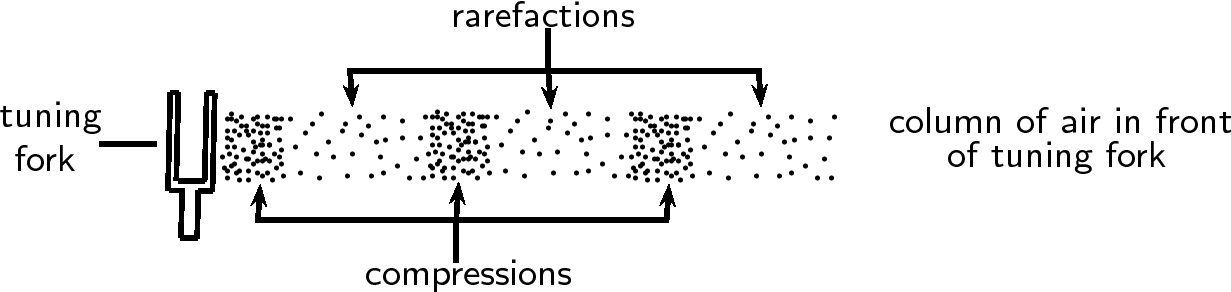
\includegraphics[width=0.7\columnwidth]{col11305.imgs/m38783_PG11C4_010.png} % m38783;PG11C4\_010.png;;;6.0;8.5;
      \vspace{2pt}
    \vspace{\rubberspace}\par \begin{cnxcaption}
	  \small \textbf{Figure 8.6: }Sound waves are pressure waves and need a medium through which to travel.
	\end{cnxcaption}
    \vspace{.1in}
    \rule[.1in]{\figurerulewidth}{.005in} \\
    \end{center}
 \end{figure}       
\label{m38783*notfhsst!!!underscore!!!id409}
\begin{tabular}{cc}
	   \hspace*{-50pt}\raisebox{-8 mm}{ 
\includegraphics[width=0.5in]{col11305.imgs/pstip2.png}  }& 
	\begin{minipage}{0.85\textwidth}
	\begin{note}
      {tip: }A sound wave is different from a light wave.
      \label{m38783*id293489}\begin{itemize}[noitemsep]
            \label{m38783*uid19}\item A sound wave is produced by an oscillating object while a light wave is not.
\end{itemize}
      \label{m38783*id293505}Also, because a sound wave is a mechanical wave (i.e. that it needs a medium) it is not capable of traveling through a vacuum, whereas a light wave can travel through a vacuum.\par 
	\end{note}
	\end{minipage}
	\end{tabular}
	\par
\label{m38783*notfhsst!!!underscore!!!id415}
\begin{tabular}{cc}
	   \hspace*{-50pt}\raisebox{-8 mm}{ 
\includegraphics[width=0.5in]{col11305.imgs/pstip2.png}  }& 
	\begin{minipage}{0.85\textwidth}
	\begin{note}
      {tip: }A sound wave is a pressure wave. This means that regions of high pressure (compressions) and low pressure (rarefactions) are created as the sound source vibrates. These compressions and rarefactions arise because the source vibrates longitudinally and the longitudinal motion of air produces pressure fluctuations.
	\end{note}
	\end{minipage}
	\end{tabular}
	\par
      \label{m38783*id293519}Sound will be studied in more detail in Sound\footnote{\raggedright{}"Sound - Grade 10 (11) [CAPS]" <http://http://cnx.org/content/m37912/latest/>}.\par 
    \label{m38783*cid8}
            \subsection{ Summary - Longitudinal Waves}
            \nopagebreak
      \label{m38783*id293550}\begin{enumerate}[noitemsep, label=\textbf{\arabic*}. ] 
            \label{m38783*uid20}\item A longitudinal wave is a wave where the particles in the medium move parallel to the direction in which the wave is travelling.
\label{m38783*uid21}\item Longitudinal waves consist of areas of higher pressure, where the particles in the medium are closest together (compressions) and areas of lower pressure, where the particles in the medium are furthest apart (rarefactions).
\label{m38783*uid22}\item The wavelength of a longitudinal wave is the distance between two consecutive compressions, or two consecutive rarefactions.
\label{m38783*uid23}\item The relationship between the period ($T$) and frequency ($f$) is given by
\label{m38783*id293619}\nopagebreak\noindent{}
    \begin{equation}
    T=\frac{1}{f}\phantom{\rule{3pt}{0ex}}\mathrm{or}\phantom{\rule{3pt}{0ex}}f=\frac{1}{T}\tag{8.8}
      \end{equation}
    \label{m38783*uid24}\item The relationship between wave speed ($v$), frequency ($f$) and wavelength ($\lambda $) is given by
\label{m38783*id293694}\nopagebreak\noindent{}
    \begin{equation}
    v=f\lambda \tag{8.9}
      \end{equation}
    \label{m38783*uid25}\item Graphs of position vs time, velocity vs time and acceleration vs time can be drawn and are summarised in figures
\label{m38783*uid26}\item Sound waves are examples of longitudinal waves. The speed of sound depends on the medium, temperature and pressure. Sound waves travel faster in solids than in liquids, and faster in liquids than in gases. Sound waves also travel faster at higher temperatures and higher pressures.
\end{enumerate}
   \label{m38783*cid9}
            \subsection{ Exercises - Longitudinal Waves}
            \nopagebreak
      \label{m38783*id293753}\begin{enumerate}[noitemsep, label=\textbf{\arabic*}. ] 
            \label{m38783*uid27}\item Which of the following is not a longitudinal wave?
\label{m38783*id293768}\begin{enumerate}[noitemsep, label=\textbf{\alph*}. ] 
            \label{m38783*uid28}\item seismic P-wave
\label{m38783*uid29}\item light
\label{m38783*uid30}\item sound
\label{m38783*uid31}\item ultrasound
\end{enumerate}
                \label{m38783*uid32}\item Which of the following media can sound not travel through?
\label{m38783*id293834}\begin{enumerate}[noitemsep, label=\textbf{\alph*}. ] 
            \label{m38783*uid33}\item solid
\label{m38783*uid34}\item liquid
\label{m38783*uid35}\item gas
\label{m38783*uid36}\item vacuum
\end{enumerate}
                \label{m38783*uid37}\item Select a word from Column B that best fits the description in Column A:
    % \textbf{m38783*id293899}\par
          \begin{table}[H]
    % \begin{table}[H]
    % \\ 'id2916739' '1'
        \begin{center}
      \label{m38783*id293899}
    \noindent
    \tabletail{%
        \hline
        \multicolumn{2}{|p{\mytableboxwidth}|}{\raggedleft \small \sl continued on next page}\\
        \hline
      }
      \tablelasttail{}
      \begin{xtabular}[t]{|l|l|}\hline
        \textbf{Column A} &
        \textbf{Column B}% make-rowspan-placeholders
     \tabularnewline\cline{1-1}\cline{2-2}
      %--------------------------------------------------------------------
        waves in the air caused by vibrations &
        longitudinal waves% make-rowspan-placeholders
     \tabularnewline\cline{1-1}\cline{2-2}
      %--------------------------------------------------------------------
        waves that move in one direction, but medium moves in another &
        frequency% make-rowspan-placeholders
     \tabularnewline\cline{1-1}\cline{2-2}
      %--------------------------------------------------------------------
        waves and medium that move in the same direction &
        white noise% make-rowspan-placeholders
     \tabularnewline\cline{1-1}\cline{2-2}
      %--------------------------------------------------------------------
        the distance between consecutive points of a wave which are in phase &
        amplitude% make-rowspan-placeholders
     \tabularnewline\cline{1-1}\cline{2-2}
      %--------------------------------------------------------------------
        how often a single wavelength goes by &
        sound waves% make-rowspan-placeholders
     \tabularnewline\cline{1-1}\cline{2-2}
      %--------------------------------------------------------------------
        half the difference between high points and low points of waves &
        standing waves% make-rowspan-placeholders
     \tabularnewline\cline{1-1}\cline{2-2}
      %--------------------------------------------------------------------
        the distance a wave covers per time interval &
        transverse waves% make-rowspan-placeholders
     \tabularnewline\cline{1-1}\cline{2-2}
      %--------------------------------------------------------------------
        the time taken for one wavelength to pass a point &
        wavelength% make-rowspan-placeholders
     \tabularnewline\cline{1-1}\cline{2-2}
      %--------------------------------------------------------------------
         &
        music% make-rowspan-placeholders
     \tabularnewline\cline{1-1}\cline{2-2}
      %--------------------------------------------------------------------
         &
        sounds% make-rowspan-placeholders
     \tabularnewline\cline{1-1}\cline{2-2}
      %--------------------------------------------------------------------
         &
        wave speed% make-rowspan-placeholders
     \tabularnewline\cline{1-1}\cline{2-2}
      %--------------------------------------------------------------------
    \end{xtabular}
      \end{center}
    \begin{center}{\small\bfseries Table 8.1}\end{center}
    \begin{caption}{\small\bfseries Table 8.1}\end{caption}
\end{table}
    \par
          \label{m38783*uid38}\item A longitudinal wave has a crest to crest distance of 10~m. It takes the wave 5 s to pass a point.
\label{m38783*id294078}\begin{enumerate}[noitemsep, label=\textbf{\alph*}. ] 
            \label{m38783*uid39}\item What is the wavelength of the longitudinal wave?
\label{m38783*uid40}\item What is the speed of the wave?
\end{enumerate}
                \label{m38783*uid41}\item A flute produces a musical sound travelling at a speed of $320\phantom{\rule{2pt}{0ex}}\mathrm{m}\ensuremath{\cdot}\mathrm{s}{}^{-1}$. The frequency of the note is 256 Hz. Calculate:
\label{m38783*id294137}\begin{enumerate}[noitemsep, label=\textbf{\alph*}. ] 
            \label{m38783*uid42}\item the period of the note
\label{m38783*uid43}\item the wavelength of the note
\end{enumerate}
                \label{m38783*uid44}\item A person shouts at a cliff and hears an echo from the cliff 1~s later. If the speed of sound is $344\phantom{\rule{2pt}{0ex}}\mathrm{m}\ensuremath{\cdot}\mathrm{s}{}^{-1}$, how far away is the cliff?\newline
\label{m38783*uid45}\item A wave travels from one medium to another and the speed of the wave decreases. What will the effect be on the ... (write only \textsl{increases, decreases} or \textsl{remains the same})
\label{m38783*id294228}\begin{enumerate}[noitemsep, label=\textbf{\alph*}. ] 
            \label{m38783*uid46}\item wavelength?
\label{m38783*uid47}\item period?
\end{enumerate}
                \end{enumerate}
  \label{m38783**end}
  \label{e91550bed2a1600e0ddb2572d580bf8e**end}
\par \raisebox{-5 pt}{
\includegraphics[width=0.5cm]{col11305.imgs/summary_www.png}} Find the answers with the shortcodes:
 \par \begin{tabular}[h]{cccccc}
 (1.) l2d  &  (2.) l2v  &  (3.) l2w  &  (4.) l2f  &  (5.) l2G  &  (6.) l27  &  (7.) l2A  & \end{tabular}
